\problemname{Lifting Walls}
The local building firm needs your help. They are building
an apartment building where the walls are prefabricated and lifted
in place using cranes. The building firm has located $n$ possible
locations for cranes, and needs to choose some of these so that
the center of each wall can be reached by at least one crane. The
cranes are quite expensive, so they want to use as few of them as
possible. A crane can reach a wall if the wall's center is at most a
distance $r$ away.

The house that is to be built is rectangular with a length $l$ and
width $w$.

\section*{Task}
Find the minimum number of cranes required to reach the center of all four walls.

\begin{figure}[h]
    \centering
    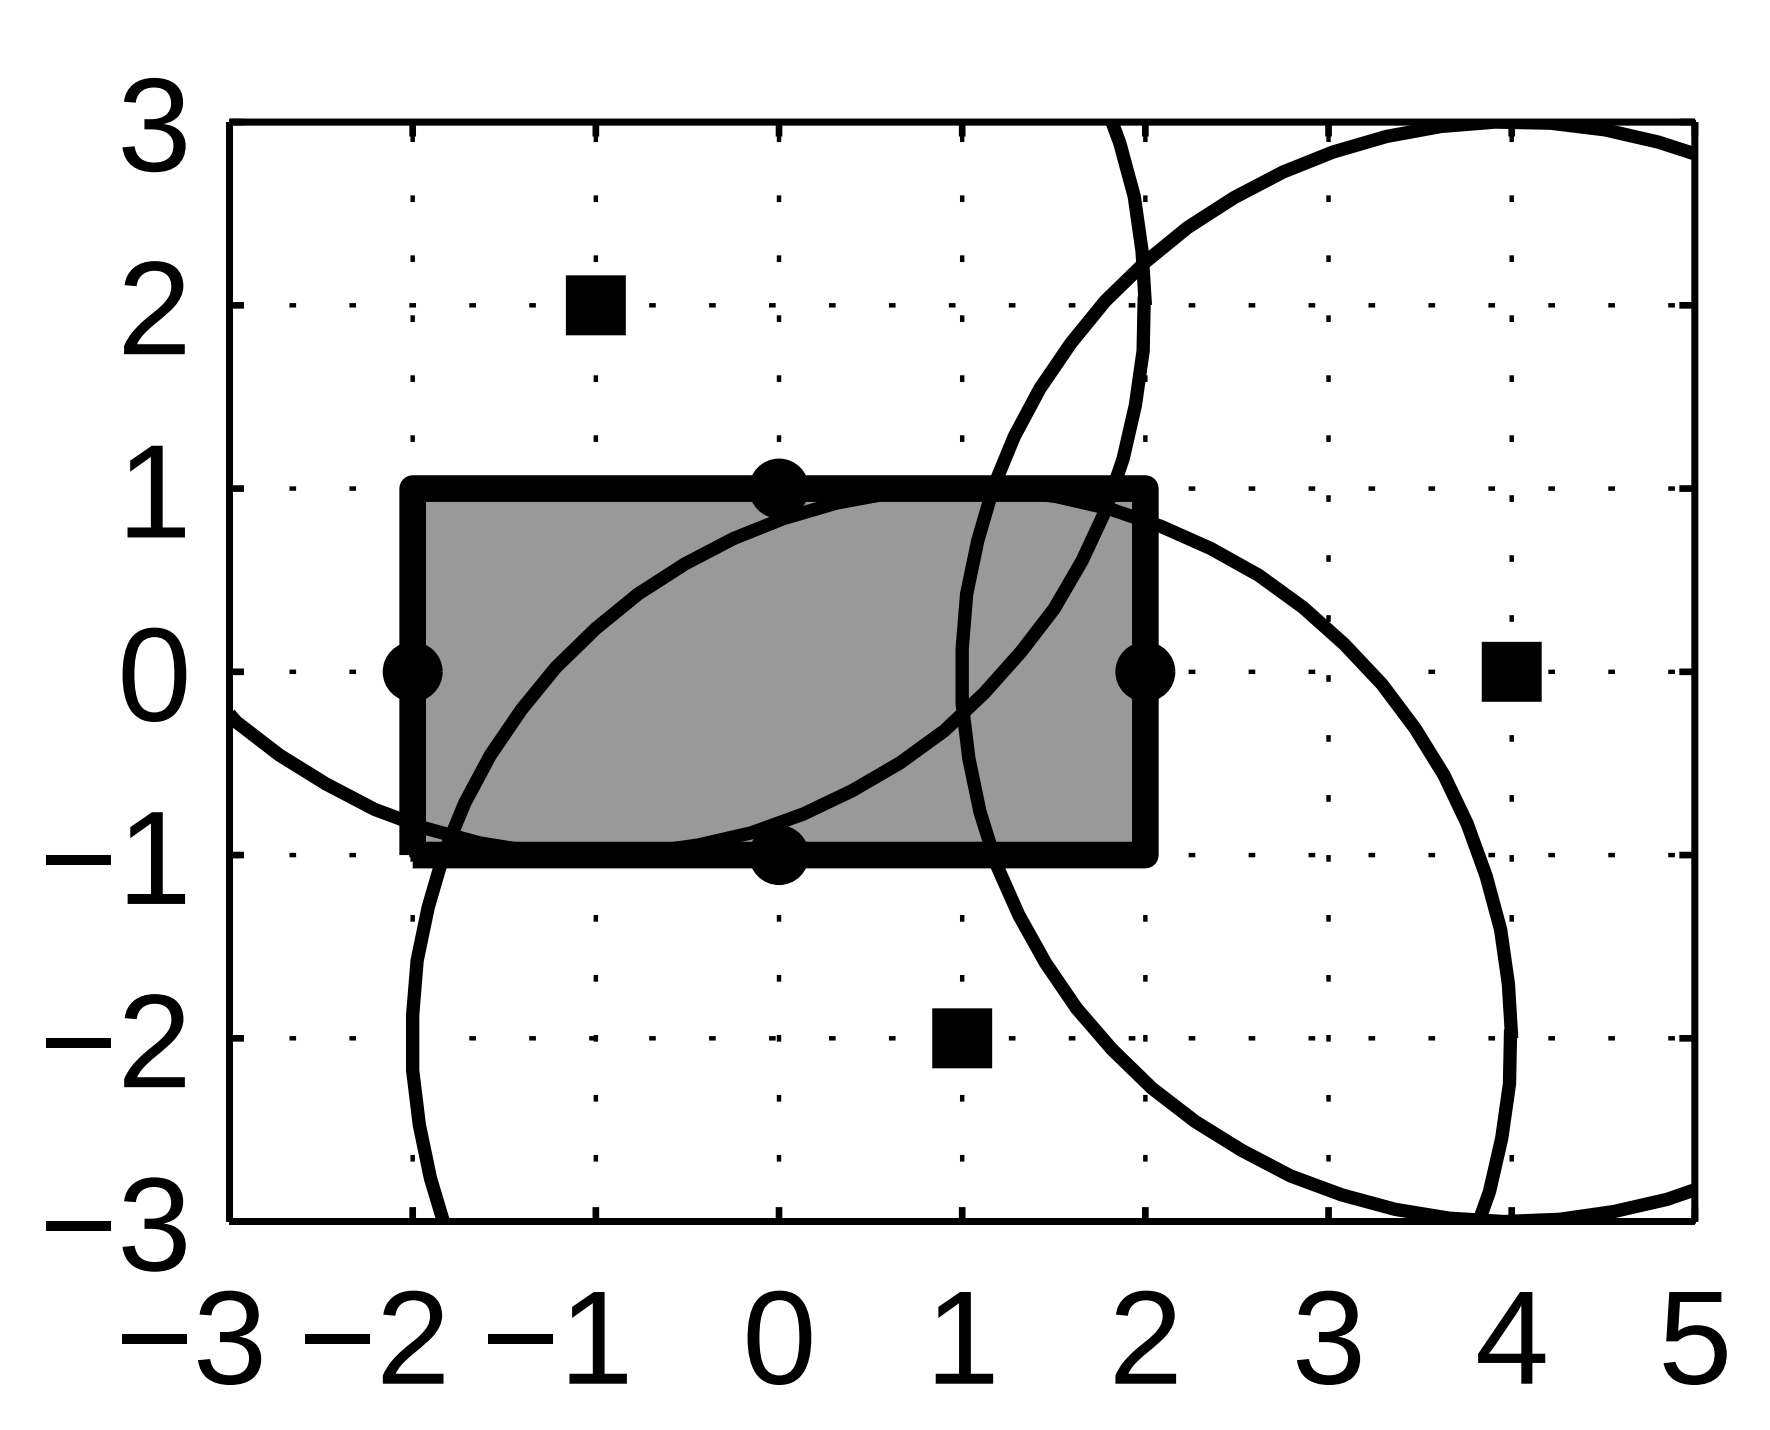
\includegraphics[width=0.3\textwidth]{walls.png}
    \caption{This example corresponds to sample input 1.}
\end{figure}

\section*{Input}
The first line of input contains four space-separated positive integers $l$, $w$, $n$ and $r$, all at most $30$.
$l$ and $w$ denote the length and width of the house, $n$ denotes the number of possible crane locations, and $r$ denotes the reaching distance of each crane.

This is followed by $n$ lines, each containing two integers $x$ and $y$ ($-100 \le x, y \le 100$), denoting a possible location for a crane.
The coordinate system has its origin in the center of the building and the $x$-coordinate along the length of the house.
The walls thus have their centers at $(x, y) = (-l/2, 0),(l/2, 0),(0, -w/2),(0, w/2)$.

\section*{Output}
Output one integer, the minimum number of cranes required to reach all wall segments, or \texttt{Impossible} if not
all wall segments can be reached.
